\section{Additional properties} %TODO move all properties to more appropriate places in thesis (eg coherent directly after the st/prf relation)?
In this section we look at some other properties of argumentation frameworks.\cl

\subsection{Finitary argumentation frameworks}
In the course of this thesis we only discussed argumentation frameworks that have a finite number of attacks. These are called \emph{finitary} as defined in \cite{Dung}.\hl

\textbf{Definition ?.} Let $F=(A,R)$ be an argumentation framework. $F$ is \emph{fintary} iff for each argument $a\in A$, there are only finitely many arguments in $R$ that attack $a$.\cl %graph impossible for non-finitary framework, because infinite amout of arguments/recursion needed

\subsection{Well-founded argumentation frameworks}
If an argumentation framework has exactly one extension that is grounded, preferred and stable, it is called a \emph{well-founded} argumentation framework (\cite{Dung}).\hl %TODO make sentence better

\textbf{Definition ?.} Let $F$ be an argumentation framework. It is called \emph{well-founded} iff there is no infinite sequence $a_0,a_1, ... , a_n, ...$ such that for each $i$, $a_{i+1}$ attacks $a_i$.\hl %meaning there is no cycle/no infinite number of arguments

\textbf{Example ?.} Let $F=(A,R)$ be an argumentation framework such that $A=\{a,b,c,d\}$ and $R=\{(a,b),(a,c),(a,d)\}$.\hl

\FloatBarrier
\begin{figure}[!h]
	\centering
	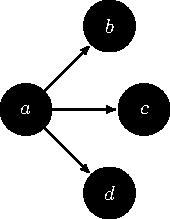
\includegraphics[scale=1.5]{graphs/wfex.pdf}
	\caption{A well-founded argumentation framework.}
\end{figure}
\FloatBarrier

 Therefore $F$ is well-founded.
Because $adm(F)=\{\emptyset, \{a\}\}$, it is obvious that $\{a\}$ is the only stable, complete (and therefore grounded) and preferred extension.

\subsection{Coherent argumentation frameworks}
If there are no ``anomalies'' in an argumentation framework it is called \emph{coherent} which was defined in \cite{Dung} as follows:\hl

\textbf{Definition ?.}  Let $F$ be an argumentation framework.\\
1) It is called \emph{coherent} if $prf(F)=st(F)$.\\
2) It is called \emph{relatively grounded} iff $gr(F)=\bigcap\limits prf(F)$.\hl

Because $\emptyset$ can never be a stable extension, an argumentation framework $F$ where $\emptyset\in prf(F)$ can not be coherent. Since there is always at least one preferred extension in an argumentation framework, it follows that a coherent argumentation framework has at least one stable extension.\cl

\subsection{Controversial argumentation frameworks}
\cite{Dung} defines the proptery of controversiality, an argument being \emph{controversial} if it both indirectly defends and indirectly attacks another argument, as follows:\hl

\textbf{Definition ?.} If there exists a finite sequence of arguments $a_0,...,a_{2n+1}$, we say an argument $a$ is \emph{indirectly attacked} by an argument $b$ if 1) $a=a_0$ and $b=a_{2n+1}$ and 2) for each $i$, $0\le i\le 2n$, $(a_{i+1},a_i)\in R$. If there exists a finite sequence of arguments $a_0,...,a_{2n}$ we say an argument $a$ is \emph{indirectly defended} by an argument $b$ if 1) $a=a_0$ and $b=a_{2n}$ and 2) for each $i$, $0\le i\le 2n$, $(a_{i+1},a_i)\in R$. An argument $b$ is \emph{controversial} wrt to an argument $a$ if $b$ indirectly attacks $a$ and indirectly defends $a$. An argument is called \emph{controversial} if it is controversial wrt some argument.\cl

Based on that definition, \cite{Dung} also contains the definition for an argumentation framework being \emph{uncontroversial}:\hl %TODO replace ``that definition'' with Definition X.

\textbf{Definition ?.} 1) An argumentation framework is \emph{uncontroversial} if none of its arguments is controversial. 2) An argumentation framework is \emph{limited controversial} if there exists no infinite sequence of arguments $a_0,...,a_n,...$ such that $a_{i+1}$ is controversial wrt $a_i$.\cl

\textbf{Example ?.} Let $F=(A,R)$ be an argumentation framework, where $A=\{a,b,c,d,e\}$ and $R=\{(b,a),(c,b),(d,c),(e,b)\}$.\hl

\FloatBarrier
\begin{figure}[!h]
	\centering
	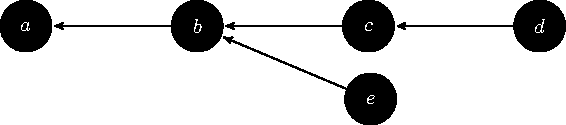
\includegraphics[width=\linewidth]{graphs/ind.pdf}
	\caption[Indirect attacks and defences]{Argumentation framework containing indirect attacks and defences.}
\end{figure}
\FloatBarrier

As we can see there is a finite sequence $a_0,...,a_{2n+1}$ that satisfies the conditions for \emph{indirect attacks}: $a,b,c,d$. As $d$ attacks the ``defender'' of $a$ against $b$, $c$, we can say $d$ indirectly attacks $a$.\hl
There are three finite sequences $a_0,...,a_{2n}$ that satisfy the conditions for \emph{indirect defences}. 1) $a,b,c$, 2) $b,c,d$ and 3) $a,b,e$, so that we can say $c$ and $e$ indirectly defend $a$ and that $d$ indirectly defends $b$.\hl
Since there is no argument that indirectly attacks and indirectly defends the same argument, thus being controversial, $F$ is \emph{uncontroversial}.\hl
Now suppose there was an additional attack $(c,e)$, such that $R=\{(b,a),(c,b),(d,c),(e,b),(c,e)\}$, resulting in the following graph:\hl

\FloatBarrier
\begin{figure}[!h]
	\centering
	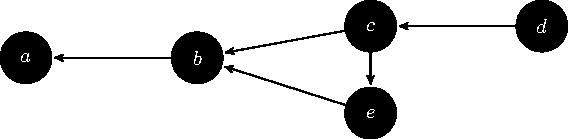
\includegraphics[width=\linewidth]{graphs/cont.pdf}
	\caption{A controversial argumentation framework.}
\end{figure}
\FloatBarrier

$a,b,e,c,d$ would result in $d$ indirectly defending $a$, but since $d$ also indirectly attacks $a$, $d$ would be \emph{controversial}, so that $F$ wouldn't be uncontroversial.\hl
$F$ is \emph{limited controversial} in both cases, since there are no infinite sequences of arguments in this example.\cl

%TODO evaluate if enough and if it is even needed
%\subsection{Property relationships}
%As before with extensions we will now take a look at how the properties mentioned in this chapter relate to each other.\hl

%In \cite{Dung} the following relationships are mentioned:\\
%1) Uncontroversial argumentation frameworks are always limited controversial, but not vice versa.\\
%2) Limited controversial argumentation frameworks are always coherent.\\
%3) Uncontroversial argumentation frameworks are always coherent and relatively grounded.\hl